\chapter{Perceptual Quality}\label{chap:02}
\begin{chapter-abstract}
Here I give an overview on the concept of \ac{QoE}.
This is basically Psychophysics (Perception): Blauert, Moeller, Jekosch and Raake.
I present standard assessment methods (\ac{ACR}, \ac{MUSHRA} etc.)and the underlying/implicit assumption for user studies).
However, the main focus on \textit{higher level} concepts (Moeller, ARCU and Geerts), which propose a more holistic approach towards \ac{QoE} and consider time and repeated usage.
At the end I will discuss, how \ac{QoE} relates to concepts of Utility, Acceptability, Satisfaction and Service Quality (needed in chap 4).
Those concept are important from the business perspective.

I should here include also some technical examples why \ac{QoE} is important for \ac{IP}-based networks.
Specialized methods for assessment of temporal effects / performance fluctuations are presented in \autoref{chap:04}.
\end{chapter-abstract}

\section{Perception and Psychophysics}
%\item What is perception?
%\item What is psychophysics? Where does it come from?
Human use their senses, \ie perceptual organs, to perceive the events of their environment.
Based upon perceived events an internal model is created and updated, which incorporates knowledge about the environment and thus reality.
This model is then used to plan actions and updated, when new information including perceptual events are processed.
%\cite[p. 4]{blauert_spatial_1996}: "Auditory events, at first relatively diffuse in their locatedness, become more precisely defined spatially; the correspondence to the visual world and to other senses also become more precise."

%\item Perceptual Event (with Sensory Processing [QoE Book Chap 2]): A physical event may(!) trigger a
%\item (Physical) Event: An observable occurrence with time, location, character [Whitepaper] -> Duration? [me]
A \emph{perceptual event} occurs in a human observer occurs, when a \emph{physical event} stimulates a sensory organ~\cite{blauert_spatial_1996}.
A physical event is an observable occurrence in time, location and character~\cite{callet_qualinet_2013}.
One example of a physical event is a sound event that reaches the ear results in an auditory event in the observer (see \autoref{img:chap02:auditory-event}).
Because the perceptual event occurs inside the observer, also due to perceptual and mental processing, it cannot observed directly.
A perceptual event can only be described by the observer by comparing the perception to other known features and express it.

\begin{figure}
%	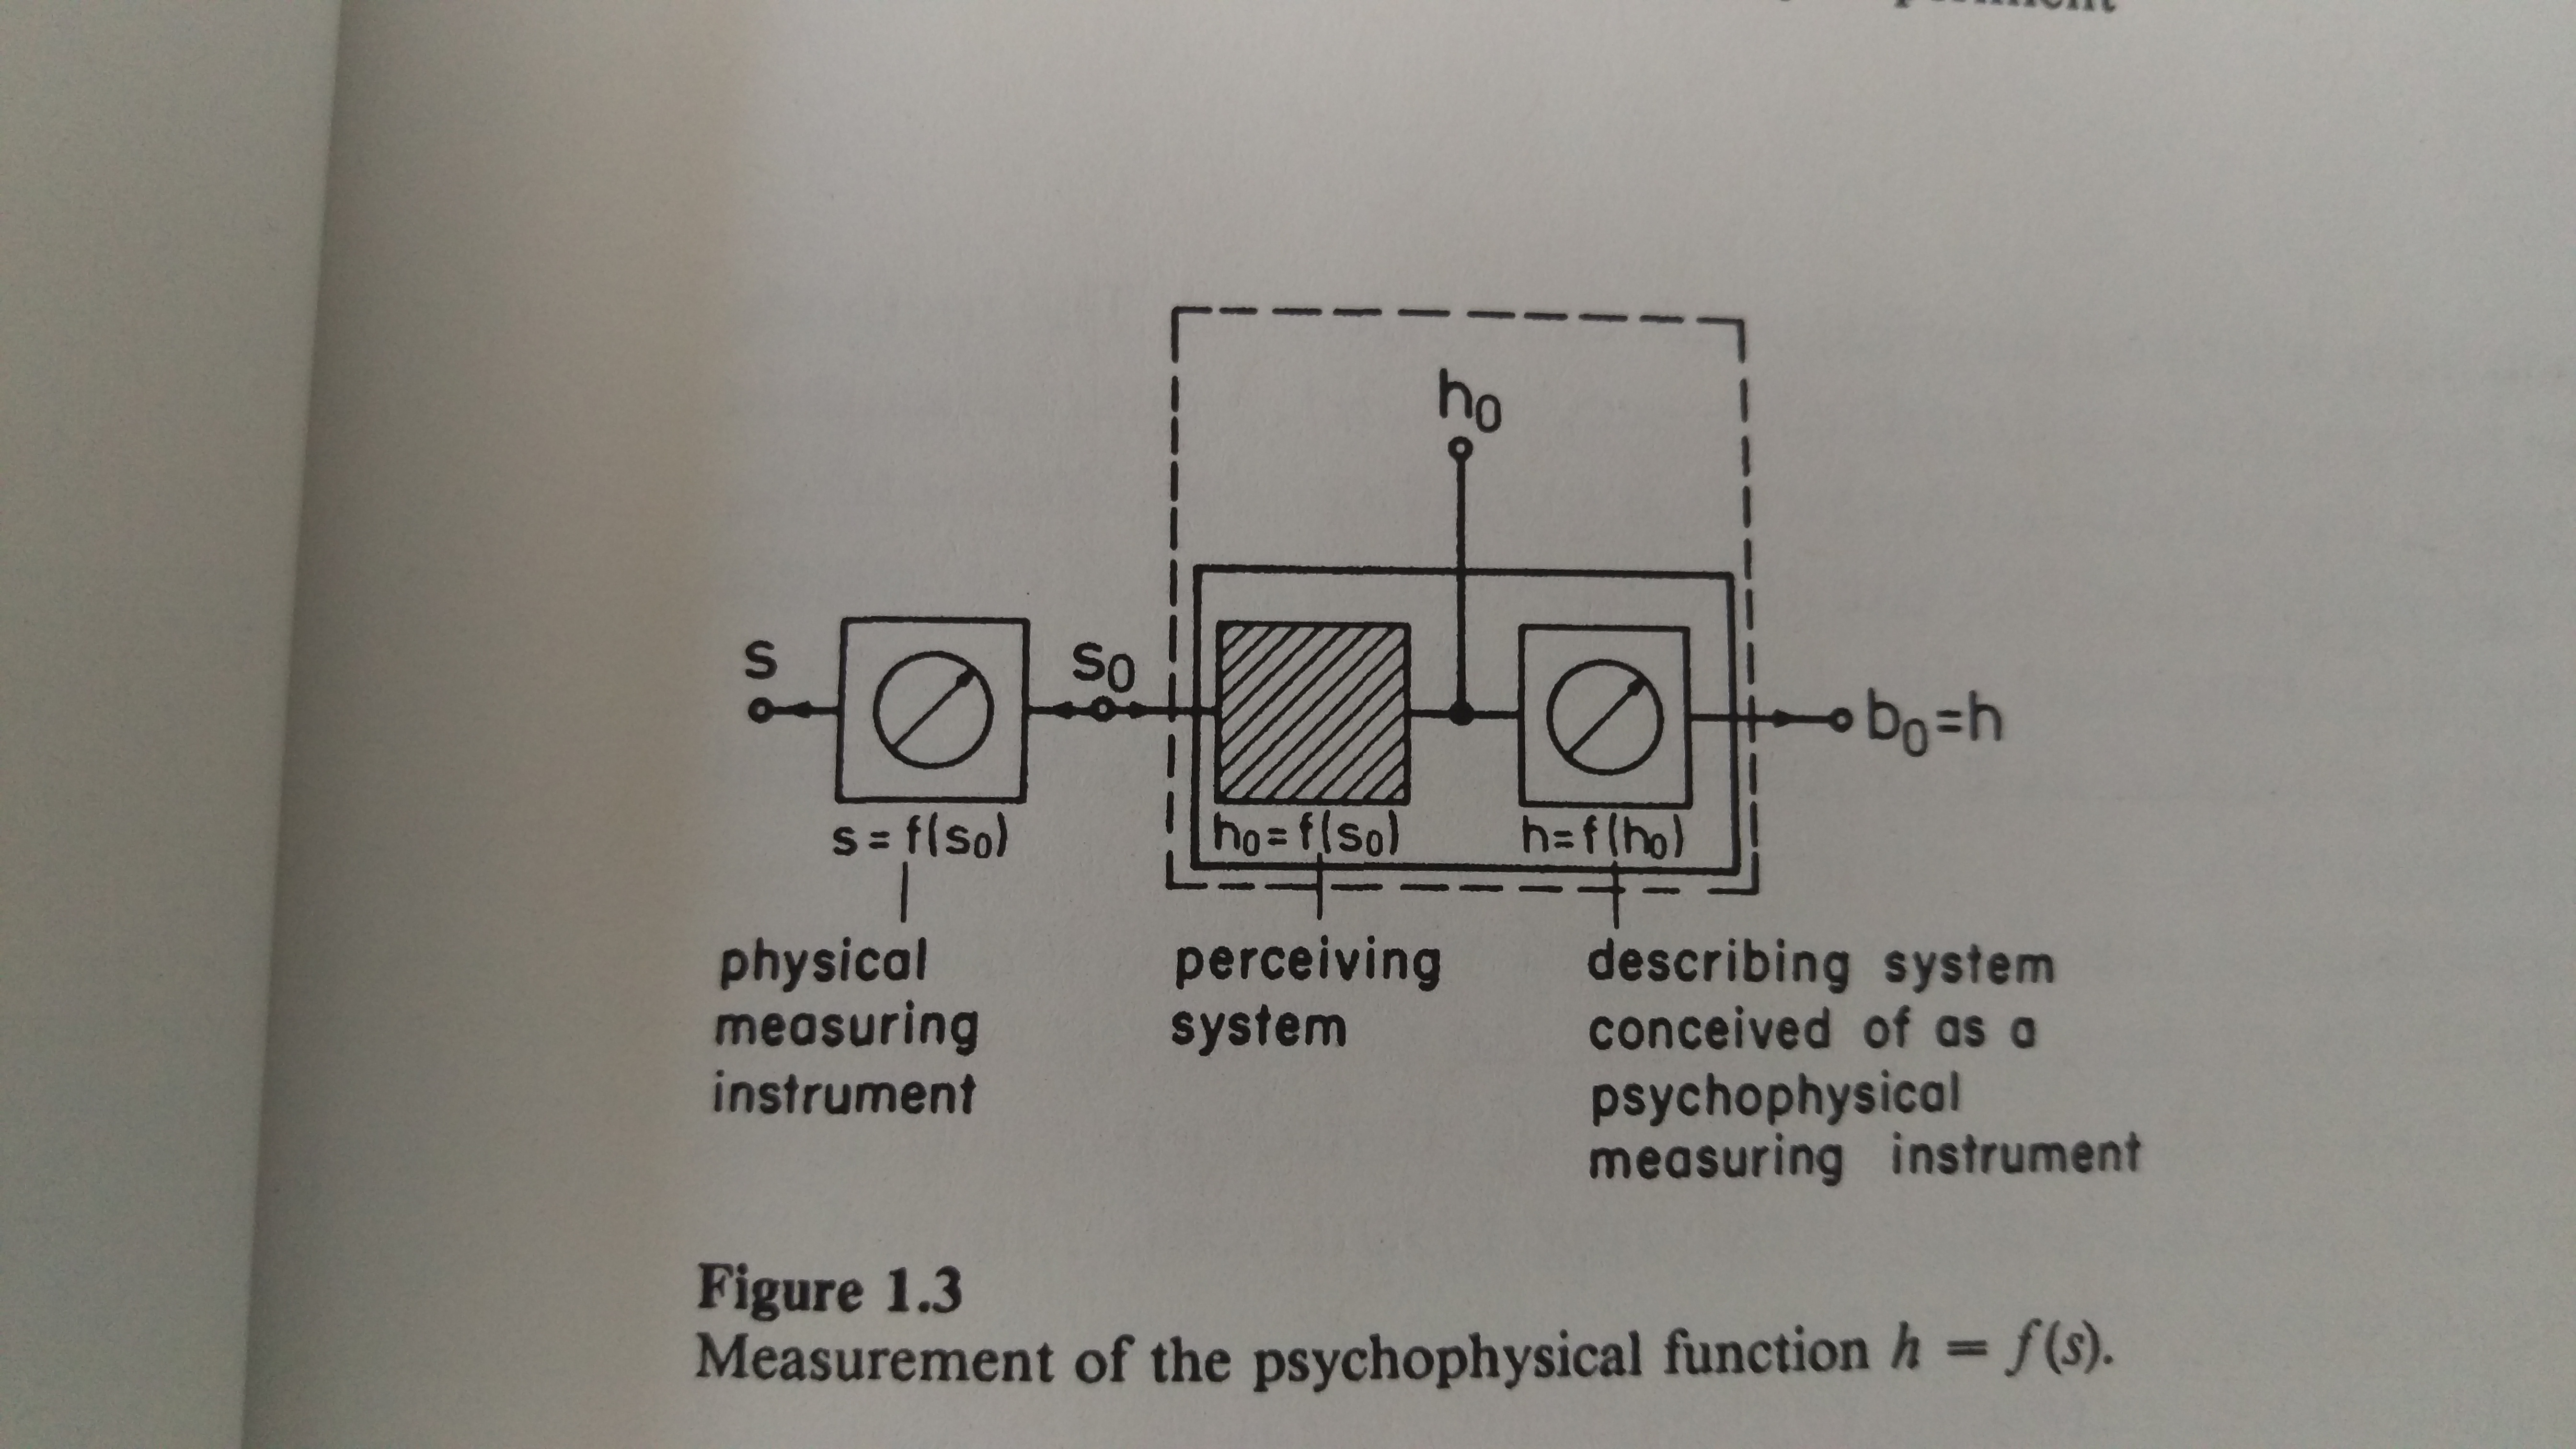
\includegraphics[width=1\textwidth]{fig/perceptual-event}
	\caption{Blauerts Perceptual event (Blauert stuff)}	
	\label{img:chap02:auditory-event}
\end{figure}
%Blauert ergodic system p.11 mittig

%\item Definition of physical observable things may lead to perception AND may be memorized.
By measuring the properties of a physical event and relating those measurements to the description of the perceptual events psychometric functions can be derived.
%\item Inherent assumption: perception is more or less reproducible: humans perceive similar
The description of a physical event and their perception must not necessarily be identical for different observers as each observer describes his individual perceptual event~\cite[p. 11]{blauert_spatial_1996}.
A psychophysical experiment is considered \emph{objective}, if the results are reproducible, independent if one subject is measured repeatedly or multiple subjects are used, \ie the system is ergodic~\cite[p. 11]{blauert_spatial_1996}.

A physical event, also if it is not consciously results in a perceptual event, may change the internal state of an observer.
The physical event reaching the sensory organ can affect the sensitivity to following physical events.
For example a bright light consumes the amount of chemicals in the eye and thus directly following physical events consisting of light will be perceived differently by the eye.
With regard to physical events that can be perceived by the human ear similar effects occurs.
Here a sound wave reaching the one ear affects the ear nerve cells behavior and thus the perception of following sound waves changes. %Add sentence about 4ms adaption of ear cells stuff (REF)
%TODO Cocktailparty effect
That the perception of a physical event depends actually on previous physical events has already been observed by Weber~\cite{Weber-Fechner} leading to the notion \ac{JND} for the perceptability of physical changes.
The perception of different physical events is not only affected by the temporal order, but temporal close physical events may grouped together and form one perceptual event.%TODO REF
This perceptual event can then not split directly into the physical events by the observer.

Not only changes in the sensory organs affect perception of physical events.
One example for this is the so-called \emph{cocktail party effect} showing how focus affect perception.
This denotes the fact that a person can actively focus on a sound source and filter additional sound source that are not in the focus.
This allows a person to listen to one speaker in a room with several parallel speakers.

A psychophysical experiment is conducted by presenting one or more physical events as stimuli to one or more observers.
Each individual observer derives the description of his perceptual event by translating it to \todo{XXX}.
The description can be expressed in a quantitative form by selecting the best fitting answer from a pre-defined set or in a free form.
Whereas in the first case the encoding is conducted by an observer himself, in the latter case the encoding open by the observer.
The description task requires that the perceptual event can be observed consciously and an \emph{active} observation process may affect the actual perception and thus perceptual event.%TODO REF
%Add training results in more differentiated perception
In addition to variations in the perception process leading to varying perception also the observation and description process is not constant.
The description process of a perceptual event may be affected by previous perceptual events that form an internal reference that is used for description (e.g., the sound is lower than the previous one), but the description process also changes over longer time spans as more information could be memorized and can be used for the description of the perceptual event.

A physical event that lead to perceptual event that cannot be observed consciously cannot be studied using this method of active reflection.
The (subconscious) reaction of an observer to a physical event can be measured by using physiological measurements.
Common examples are eye tracking, or skin conductance.
To a certain degree also reactions of the subconscious perceptual process might be observable by 
By applying \ac{EEG}, in fact, also parts of the subconscious perceptual process happening in the brain can be observed to a certain degree.

In fact, an observer cannot only describe the perceptual event, but might react to a perceived physical event.
First he will incorporate the newly acquired information provided by the new perceptual event and update his internal representation of his environment.
The observer might then actively react, so that following physical events might yield more relevant information.
For example a human listener can actively try to the direction of a sound source by actively moving his head, which will affect following perceptual events.\todo{REF}

\section{Perceptual Quality and Quality Formation Process}
The field \emph{perceptual quality}, or so-called \ac{QoE}, is a field of psychophysics focusing on the \emph{experience} due to perceptions and the resulting \emph{quality} of this experience.
Experience is overall result from the experience of perceptual events.
\begin{definition}[Experiencing]
``is the individual stream of perceptions (of feelings, sensory percepts and concepts) that occurs in a particular situation of reference.''~\citep[p. 13]{moller_quality_2014}.
\end{definition}

%Quality: Individual comparison and judgment process with perception, reflection (optional?) and description of the outcome (optional?) [whitepaper]
%\item Quality formation process
With regard to quality of an experience, and the underlying perceptual events, \cite{jekosch_voice_2005} formulates the \emph{quality formation process} as individual comparison process between the desired outcome, or expected, with the experienced outcome.
The comparison with the expectations of the experience results in a \emph{quality event}, which similar to a perceptual event can be described.
This process is shown in \autoref{img:chap02:quality-event} as extension to the perceptual event processing and description process \todo{REF previous section, blauert}.
\begin{figure}
	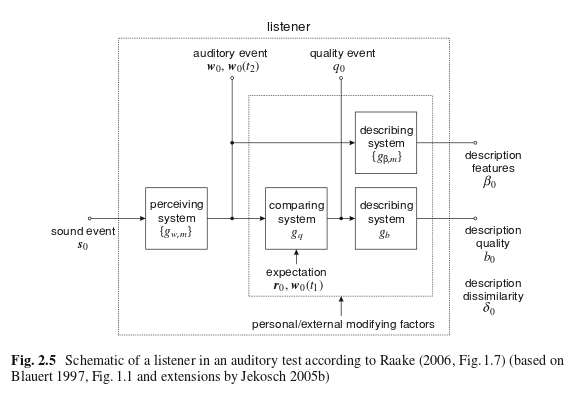
\includegraphics[width=1\textwidth]{fig/quality-event}
	\caption{Quality formation and description process as extension to the perceptual event.}
	\label{img:chap02:quality-event}
\end{figure}

It is assumed that a perceptual event is evaluated by the comparing system within an observer with regard to the \emph{quality features} of this event~\cite[cf. p. 17]{jekosch_voice_2005}.
\footnote{\cite{jekosch_voice_2005} uses the term \emph{entity} with regard to the quality formation process.
As entity does not convey a temporal component, the term \emph{event} is in this work used instead following the notion of \cite{blauert_spatial_1996} although the duration of an event is not considered there.}
The comparing system actually evaluates the difference between the \emph{perceived quality features} and the \emph{desired quality features}~\cite[p. 23]{raake_book}.

\begin{definition}[Quality Feature]
``A quality feature is a recognized and designated characteristic of an entity that is relevant to the entity's quality.''~\cite[p. 17]{jekosch_voice_2005}
\end{definition}

%, Desired nature, Internal reference, 
\cite{raake_speech_2006, moller_quality_2014} extended the \emph{quality formation process} of \cite{jekosch_voice_2005}.
Raake splits the quality formation process into three phases as shown in \autoref{img:chap02:quality-formation-process}.
The first phase contains the sensory processing depending on contextual information and predescessing perceptual events, which transforms a physical event to a perceptual event leading to the perceived characteristic.
This phase also contains reactions to the perceptual event by exploration and anticipation.
\todo{Write more about ALEX here}

\begin{figure}
	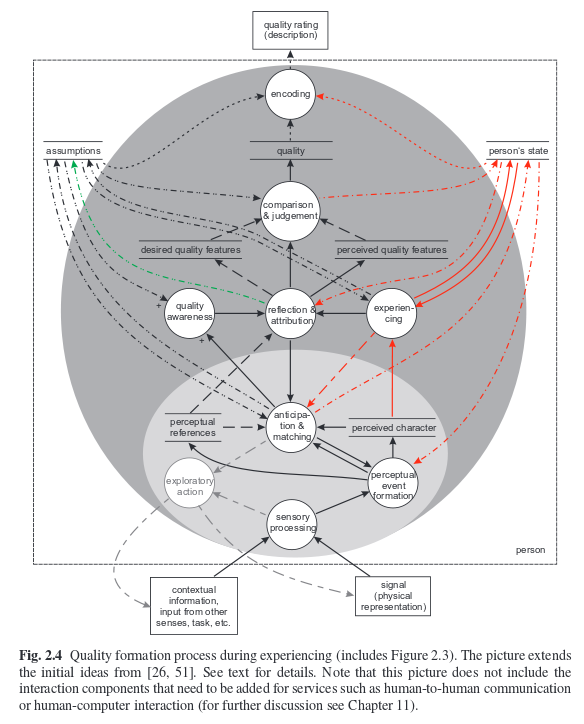
\includegraphics[width=1\textwidth]{fig/quality-formation-process}
	\caption{Quality-formation process as defined by \cite{moller_quality_2014} extending \cite{jekosch_voice_2005}.}
	\label{img:chap02:quality-formation-process}
\end{figure}

With regard to telecommunication services and multimedia systems the term \emph{perceived quality} has been extended to \acf{QoE}.
\begin{definition}[\acf{QoE}]
``is the degree of delight or annoyance of a person whose experiencing involves an application, service, or system.
It results from the person’s evaluation of the fulfillment of his or her expectations and needs with respect to the utility and / or enjoyment in the light of the person’s context, personality and current state.''~\citep[p. 21]{moller_quality_2014}.
\end{definition}

In \ac{QoE} an observer is not only regarded as a measurement instrument, but as an actor striving for a   satisfying perceived quality with regard to his expectations, requirements and needs.
In difference to an observer, who only describes an event, in QoE the perceiving human is regarded as an actor that can not only react but also proactive make decisions.

\begin{definition}[Assumed Quality]
``corresponds to the quality and quality features that users, developers, manufacturers or  service  providers assume regarding a  system, service or product that they intend to be using, or will be producing, without however grounding these assumptions on an explicit assessment of \textit{quality based on experiencing}.''~\citep[p. 20]{moller_quality_2014}.
\end{definition}

%\item Perceptual dimensions [Moeller, Raake]

%Definition: recalled quality


%Geerts - Meta-Framework merging:
%% User, Product, Use Process(Wright: identification, incorperation, identification; non-use/abondonment!), Context (cf. Mantovani)
%% WRIGHT. Micro (in one session): anticipating, connecting, interpreting, reflecting, appropiating and recounting
%% WRIGHT. Macro (over multiple sessions)



%White paper (everything relies on Pyykko!)[FAIL!, Keine Literatur!]
%% Human IF: perception + interpretation and judgment
%% System IF: Content, Media, Network, Device
%% Context IF: Temporla, Economic?, Task, Social 

%Interactive Products (Karapanos) / ICT product (Geerts)

%Moeller Diss 2009
%%NOT: ALL USERS ARE NOT EQUAL
%%NOT MINKER/Weiss
%Kilikkis QoE framework (Qo User Experience and Qo Customer Experience)
%%User, Device/System/Product, Use process (preconception; before encounter, 


\section{Influence Factors on \ac{QoE}} %or: QoE frameworks
%\item Expectations: Prior experiences, Contextual Factors, Task [Moeller, Raake] 
%\item What are related concepts: QoS, Performance?
%\item Check Geerts for broader context!
%\item Moeller DISS taxonomy

\section{Assessment Methods}
%perceptual dimensions
%\item Lab vs. field studies

%paired comparison
%speech integibility
%MUSHRA direct comparins
%ACR
%Dimenions and perceptual space
%Dimension-based stuff



%Types of judgment: expected, instantouos, retrospective.
%Assumption: average user

%\item \cite{pitrey_aligning_2011}

\section{Application of {QoE}}
\begin{itemize}
\item Practical outcome? Evaluation procedures, knowledge and Objective Models (for different purpose)
\item Approaches towards modeling: how to one create a model? What are limitations?
\item Types of judgment: momentary and retrospective
\item Where degradations come from? (production/recording, coding, transmission, reproduction)
\item Performance fluctuations: temporal effects; outlook to next chapter.
\end{itemize}

\section{Related Concepts}
\begin{itemize}
\item Definition of Utility [Kahneman and also Moeller]
\item Definition of Acceptability with regard to Service
\item Definition of Satisfaction (if required?)
\item Service quality
\end{itemize}